%! Licence = CC BY-NC-SA 4.0

%! Author = gianfluetsch
%! Date = 19. Jan 2022
%! Project = pfsec_summary

\section{Cloud Security}

\subsection{Cloud Computing}
\begin{center}
    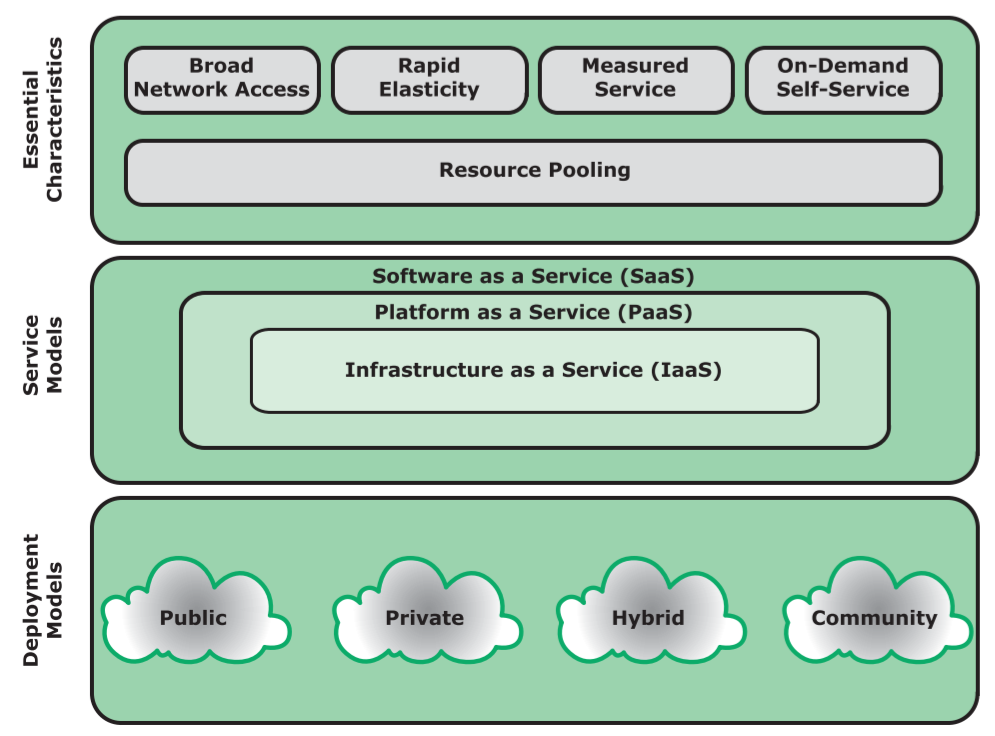
\includegraphics[width=.6\linewidth]{06-cloud_security/cloud_security}
    \vspace{-8pt}
\end{center}

\begin{itemize}
    \item \textbf{Broad network access}
    \begin{itemize}
        \item Capabilities are available over the network and accessed through standard mechanisms that promote use by heterogeneous thin or thick client platforms (e.g., mobile phones, laptops and tablets) as well as other traditional or cloud-based software services.
    \end{itemize}
    \item \textbf{Rapid elasticity}
    \begin{itemize}
        \item Cloud computing gives you the ability to expand and reduce resources according to your specific service requirement. For example, you may need a large number of server resources for the duration of a specific task. You can then release these resources upon completion of the task.
    \end{itemize}
    \item \textbf{Measured service}
    \begin{itemize}
        \item Cloud systems automatically control and optimize resource use by leveraging a metering capability at some level of abstraction appropriate to the type of service (e.g., storage, processing, bandwidth, and active user accounts). Resource usage can be monitored, controlled, and reported, providing transparency for both the provider and consumer of the utilized service.
    \end{itemize}
    \item \textbf{On-demand self-service}
    \begin{itemize}
        \item A cloud service consumer (CSC) can unilaterally provision computing capabilities, such as server time and network storage, as needed automatically without requiring human interaction with each service provider. Because the service is on demand, the resources are not permanent parts of the consumer's IT infrastructure.
    \end{itemize}
    \item \textbf{Resource pooling}
    \begin{itemize}
        \item The provider's computing resources are pooled to serve multiple CSCs using a multitenant model, with different physical and virtual resources dynamically assigned and reassigned according to consumer demand. There is a degree of location independence, in that the CSC generally has no control or knowledge of the exact location of the provided resources, but may be able to specify location at a higher level of abstraction (e.g., country, state, or datacenter). Examples of resources include storage, processing, memory, network bandwidth, and virtual machines (VMs). Even private clouds tend to pool resources between different parts of the same organization.
    \end{itemize}
\end{itemize}

\subsubsection{Cloud Service Models}

\paragraph{Software as a Service (SaaS)}
\begin{itemize}
    \item SaaS provides service to customers in the form of software, specifically application software, running on and accessible in the cloud
    \item The applications are accessible through a simple interface such as a Web browser
    \item The use of SaaS avoids the complexity of software installation, maintenance, upgrades, and patches
    \item \textit{Examples}: Microsoft 365, Salesforce, Cisco WebEx
\end{itemize}

\paragraph{Platform as a Service (PaaS)}
\begin{itemize}
    \item PaaS provides service to customers in the form of a platform on which the customer's applications can run
    \item A PaaS cloud provides useful software building blocks, plus a number of development tools, such as programming language tools, run-time environments, and other tools that assist in deploying new applications
    \item PaaS can be seen as an operating system in the cloud
    \item It is useful for an organization that wants to develop new or tailored applications while paying for the needed computing resources only as needed, and only for as long as needed
    \item \textit{Examples}: AppEngine, Engine Yard, Heroku, Microsoft Azure, Force.com, and Apache Stratos
\end{itemize}

\paragraph{Infrastructure as a Service (IaaS)}
\begin{itemize}
    \item With IaaS, the customer has access to the resources of the underlying cloud infrastructure
    \item The cloud service user does not manage or control the resources of the underlying cloud infrastructure, but has control over operating systems, deployed applications, and possibly limited control of select networking components
    \item IaaS provides virtual machines and other virtualized hardware and operating systems
    \item IaaS offers the customer processing, storage, networks, and other fundamental computing resources so the customer is able to deploy and run arbitrary software, which can include operating systems and applications
    \item \textit{Examples}: Amazon Elastic Compute Cloud, Microsoft Windows Azure, Google Compute Engine, and Rackspace
\end{itemize}

\paragraph{Responsabilities}
\begin{center}
    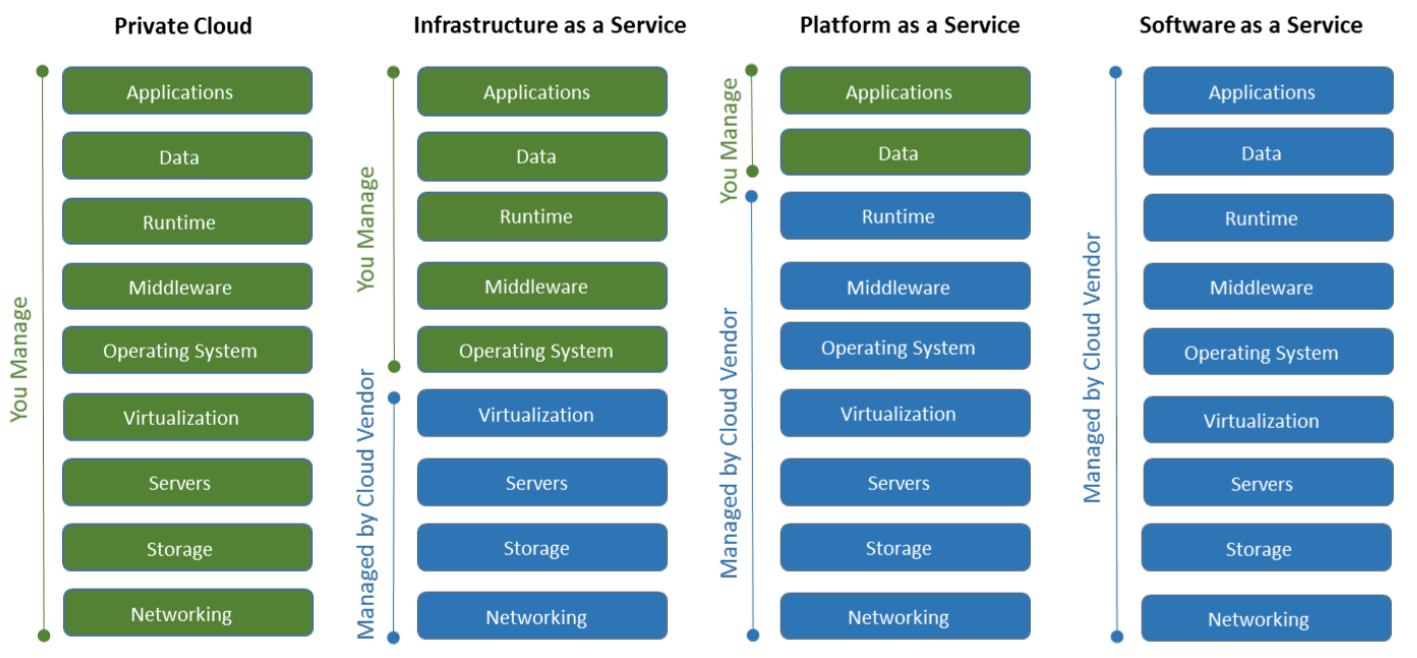
\includegraphics[width=.8\linewidth]{06-cloud_security/cloud_service_models}
    \vspace{-8pt}
\end{center}

\subsubsection{Cloud Deployment Models}
\begin{center}
    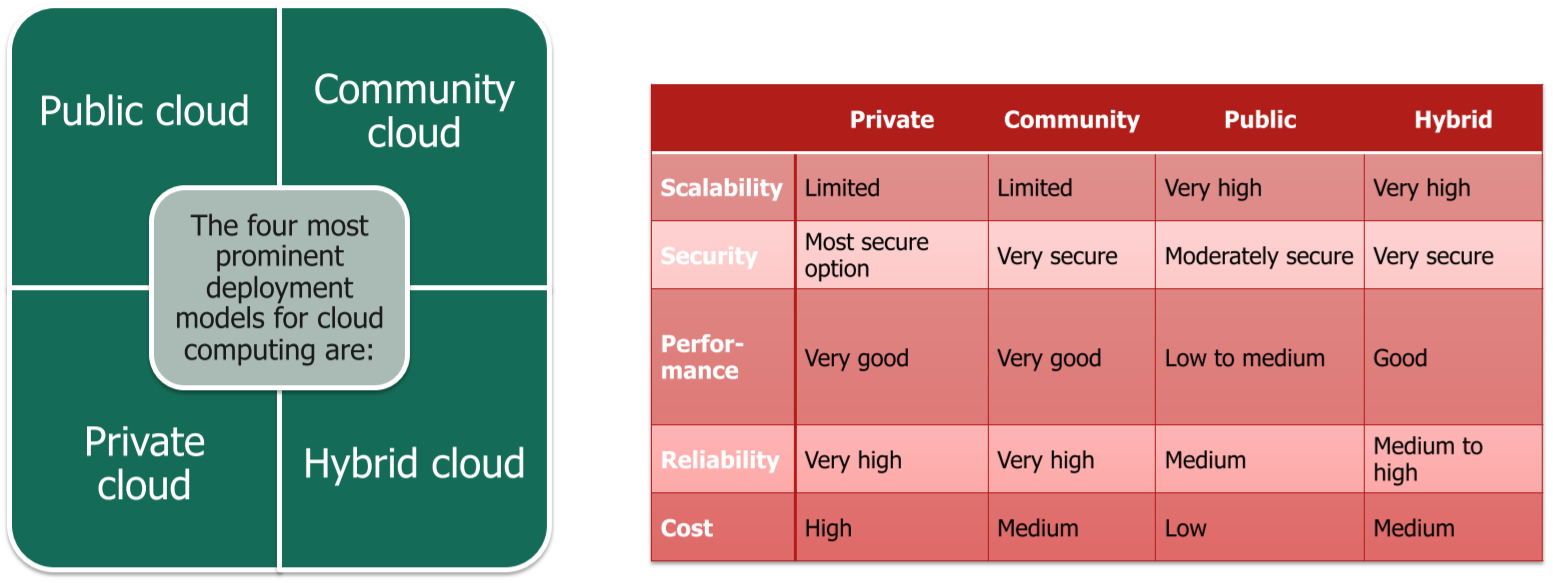
\includegraphics[width=.8\linewidth]{06-cloud_security/cloud_deployment_models}
    \vspace{-8pt}
\end{center}

\textcolor{red}{\textbf{Community based sind häufig Leute mit gleichen Interessen}\\
$\rightarrow$ die Wahrscheinlichkeit erkannt zu werden (als Person mit böser absicht) ist grösser als bei der Public Cloud}

\subsubsection{Cloud Computing Reference Architecture}
\begin{center}
    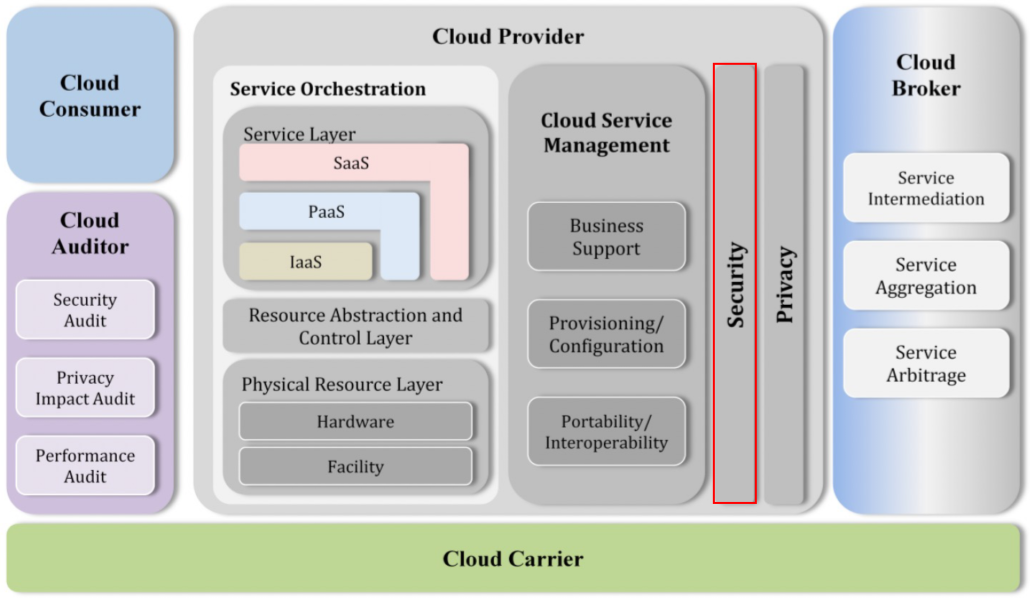
\includegraphics[width=.8\linewidth]{06-cloud_security/cloud_computing_architecture}
    \vspace{-8pt}
\end{center}

\textcolor{red}{\textbf{Security ist in allen Schichten präsent und kann somit überall "mitreden"}}\\

\begin{itemize}
    \item \textbf{Cloud Auditor}
    \begin{itemize}
        \item als begonnen wurde die Performance zu monitoren, da Performance stark mit den Kosten zusammenhängt
        \item Cloud Provider will wissen, wohin die Daten gesendet werden, damit er keine Probleme bekommen kann!
    \end{itemize}
\end{itemize}

\paragraph{Cloud Consumer}
\begin{center}
    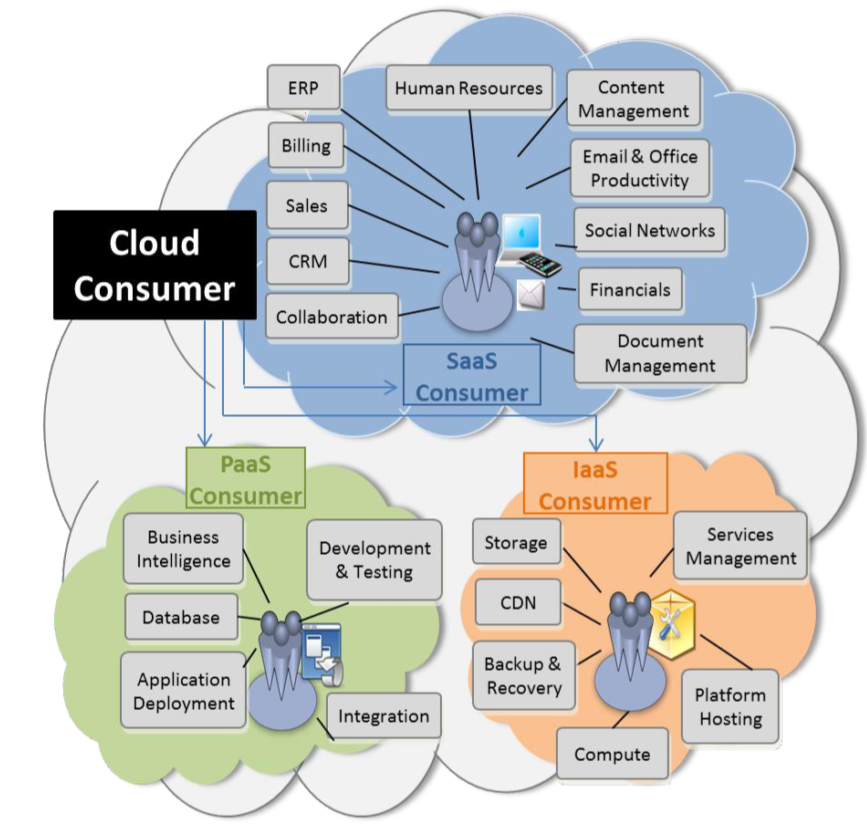
\includegraphics[width=.6\linewidth]{06-cloud_security/cloud_consumer}
    \vspace{-8pt}
\end{center}

\newpage

\subsection{Guidelines on Security \& Privacy}
\begin{table}[h]
    \centering
    \begin{tabular}{p{3cm} | p{12cm}}
        \bfseries{Areas} & \bfseries{Recommendations}\\ \hline
        Gouvernance &
        \begin{itemize}
            \item Extend organizational practices pertaining to the policies, procedures, and standards used for application development and service provisioning in the cloud, as well as the design, implementation, testing, use and monitoring of deployed or engaged services
            \item Put in place audit mechanisms and tools to ensure organizational practices are followed throughout the system lifecycle
        \end{itemize}\\
        Compliance &
        \begin{itemize}
            \item Understand the various types of laws and regulations that impose security and privacy obligations on the organization and potentially impact cloud computing initiatives, particularly those involving data location, privacy and security controls, records management, and electronic discovery requirements
            \item Review and assess the cloud provider's offerings with respect to the organizational requirements to be met and ensure that the contract terms adequately meet the requirements
            \item Ensure that the cloud provider's electronic discovery capabilities and processes do not compromise the privacy or security of data and applications
        \end{itemize}\\
        Trust &
        \begin{itemize}
            \item Ensure that service arrangements have sufficient means to allow visibility into the security and privacy controls and processes employed by the cloud provider, and their performance over time
            \item Establish clear, exclusive ownership rights over data
            \item Institute a risk management program that is flexible enough to adapt to the constantly evolving and shifting risk landscape for the lifecycle of the system
            \item Continuously monitor the security state of the information system to support on-going risk management decisions
        \end{itemize}\\
        Architecture &
        \begin{itemize}
            \item Understand the underlying technologies that the cloud provider uses to provision services, including the implications that the technical controls involved have on the security and privacy of the system, over the full system lifecycle and across all system components
        \end{itemize}\\
        Identity and Access Management &
        \begin{itemize}
            \item Ensure that adequate safeguards are in place to secure authentication, authorization, and other identity and access management functions, and are suitable for the organization
        \end{itemize}\\
        Software Isolation &
        \begin{itemize}
            \item Understand virtualization and other logical isolation techniques that the cloud provideremploys in its multitenant software architecture, and assess the risks involved for the organization
        \end{itemize}
    \end{tabular}
\end{table}

\begin{center}
    \begin{tabular}{p{3cm} | p{12cm}}
        \bfseries{Areas} & \bfseries{Recommendations}\\ \hline
        Data Protection &
        \begin{itemize}
            \item Evaluate the suitability of the cloud provider's data management solutions for the organizational data concerned and the ability to control access to data, to secure datawhile at rest, in transit, and in use, and to sanitize data
            \item Take into consideration the risk of collating organizational data with that of other organizations whose threat profiles are high or whose data collectively represent significant concentrated value
            \item Fully understand and weigh the risks involved in cryptographic key management with the facilities available in the cloud environment and the processes established by the cloud provider
        \end{itemize}\\
        Availability &
        \begin{itemize}
            \item Understand the contract provisions and procedures for availability, data backup and recovery, and disaster recovery, and ensure that they meet the organization's continuityand contingency planning requirements
            \item Ensure that during an intermediate or prolonged disruption or a serious disaster, critical operations can be immediately resumed, and that all operations can be eventually reinstituted in a timely and organized manner
        \end{itemize}\\
        Incident Response &
        \begin{itemize}
            \item Understand the contract provisions and procedures for incident response and ensure that they meet the requirements of the organization
            \item Ensure that the cloud provider has a transparent response process in place and sufficient mechanisms to share information during and after an incident
            \item Ensure that the organization can respond to incidents in a coordinated fashion with the cloud provider in accordance with their respective roles and responsibilities for the computing environment
        \end{itemize}
    \end{tabular}
\end{center}

\newpage

\subsection{Cloud Security}

\subsubsection{Cloud Security Threats}


\textbf{Abuse and abusive use of cloud computing}
\begin{itemize}
    \item Countermeasures include:
    \begin{itemize}
        \item Stricter initial registration and validation processes
        \item Enhanced credit card fraud monitoring and coordination
        \item Comprehensive inspection of customer network traffic
        \item Monitoring public blacklists for one's own network blocks\\
    \end{itemize}
\end{itemize}

\textbf{Insecure interfaces and APIs}
\begin{itemize}
    \item Countermeasures include:
    \begin{itemize}
        \item Analyzing the security model of CSP interfaces
        \item Ensuring that strong authentication and access controls are implemented in concert with encrypted transmission
        \item Understanding the dependency chain associated with the API\\
    \end{itemize}
\end{itemize}

\textbf{Malicious insiders}
\begin{itemize}
    \item Countermeasures include:
    \begin{itemize}
        \item Enforce strict supply chain management and conduct a comprehensive supplier assessment
        \item Specify human resource requirements as part of legal contract
        \item Require transparency into overall information security and management practices, as well as compliance reporting
        \item Determine security breach notification processes\\
    \end{itemize}
\end{itemize}

\textbf{Shared technology issues}
\begin{itemize}
    \item Countermeasures include:
    \begin{itemize}
        \item Implement security best practices for installation/configuration
        \item Monitor environment for unauthorized changes/activity
        \item Promote strong authentication and access control for administrative access and operations
        \item Enforce SLAs for patching and vulnerability remediation
        \item Conduct vulnerability scanning and configuration audits\\
    \end{itemize}
\end{itemize}

\textbf{Data loss or leakage}
\begin{itemize}
    \item Countermeasures include:
    \begin{itemize}
        \item Implement strong API access control
        \item Encrypt and protect integrity of data in transit and at rest
        \item Analyze data protection at both design and run time
        \item Implement strong key generation, storage and management, and destruction practices\\
    \end{itemize}
\end{itemize}

\textbf{Account or service hijacking}
\begin{itemize}
    \item Countermeasures include:
    \begin{itemize}
        \item Prohibit the sharing of account credentials between users and services
        \item Leverage strong two-factor authentication techniques where possible
        \item Employ proactive monitoring to detect unauthorized activity
        \item Understand CSP (Content Security Policy) security policies and SLAs\\
    \end{itemize}
\end{itemize}

\textbf{Unknown risk profile}
\begin{itemize}
    \item Countermeasures include:
    \begin{itemize}
        \item Disclosure of applicable logs and data
        \item Partial/full disclosure of infrastructure details
        \item Monitoring and alerting on necessary information
    \end{itemize}
\end{itemize}

\newpage

\subsubsection{OWASP Cloud-Native Application Security Top 10}
\begin{enumerate}
    \item \textbf{Insecure cloud, container or orchestration configuration}
    \begin{itemize}
        \item \textit{Examples}: Publicly open s3 bucket, Container runs as root, Container shares resources with the host (network interface, etc.), Insecure Infrastructure-as-Code (IaC) configuration\\
    \end{itemize}
    \item \textbf{Injection flaws (app layer, cloud events, cloud services)}
    \begin{itemize}
        \item \textit{Examples}: SQL injection, XXE, NoSQL injection, OS command injection, Serverless event data injection\\
    \end{itemize}
    \item \textbf{Improper authentication \& authorization}
    \begin{itemize}
        \item \textit{Examples}: Unauthenticated API access on a microservice, Over-permissive cloud IAM role, Lack of orchestrator node trust rules (e.g. unauthorized hosts joining the cluster), Unauthenticated orchestrator console access, Unauthrized or overly-permissive orchestrator access\\
    \end{itemize}
    \item \textbf{CI/CD pipeline \& software supply chain flaws}
    \begin{itemize}
        \item \textit{Examples}: Insufficient authentication on CI/CD pipeline systems, Use of untrusted images, Use of stale images, Insecure communication channels to registries, Overly-permissive registry access, Using a single environment to run CI/CD tasks for projects requiring different levels of security\\
    \end{itemize}
    \item \textbf{Insecure secrets storage}
    \begin{itemize}
        \item \textit{Examples}: Orchestrator secrets stored unencrypted, API keys or passwords stored unencrypted inside containers, Hardcoded application secrets, Poorly encrypted secrets (e.g. use of obsolete encryption methods, use of encoding instead of encryption, etc.), Mounting of storage containing sensitive information\\
    \end{itemize}
    \item \textbf{Over-permissive or insecure network policies}
    \begin{itemize}
        \item \textit{Examples}: Over-permissive pod to pod communication allowed, Internal microservices exposed to the public Internet, No network segmentation defined, End-to-end communications not encrypted, Network traffic to unknown or potentially malicious domains not monitored and blocked\\
    \end{itemize}
    \item \textbf{Using components with known vulnerabilities}
    \begin{itemize}
        \item \textit{Examples}: Vulnerable 3rd party open source packages, Vulnerable versions of application components, Use of known vulnerable container images\\
    \end{itemize}
    \item \textbf{Improper assets management}
    \begin{itemize}
        \item \textit{Examples}: Undocumented microservices \& APIs, Obsolete \& unmanaged cloud resources\\
    \end{itemize}
    \item \textbf{Inadequate 'compute' resource quota limits}
    \begin{itemize}
        \item \textit{Examples}: Resource-unbound containers, Over-permissive request quota set on APIs\\
    \end{itemize}
    \item \textbf{Ineffective logging \& monitoring (e.g. runtime activity)}
    \begin{itemize}
        \item \textit{Examples}: No container or host process activity monitoring, No network communications monitoring among microservices, No resource consumption monitoring to ensure availability of critical resources, Lack of monitoring on orchestration configuration propagation and stale configs
    \end{itemize}
\end{enumerate}

\newpage

\subsubsection{Typical Cloud Security as a Service}
\begin{enumerate}
    \item Identity and access management (IAM)
    \item Data loss prevention
    \item Web security
    \item E-mail security
    \item Security assessments
    \item Intrusion management
    \item Security information and event management
    \item Encryption
    \item Business continuity and disaster recovery
    \item Network security
\end{enumerate}